\documentclass[12pt]{article}

\usepackage{amsmath}
\usepackage{amssymb}
\usepackage{calc}
\usepackage{units}
\usepackage{graphicx}
\usepackage[pdftex]{hyperref}
\usepackage{subfig}
\usepackage[margin=1in]{geometry}
\usepackage{listings}
\usepackage[numbers,sort&compress]{natbib}
\usepackage{bm}
\usepackage{paralist}
\usepackage[draft]{fixme}
\usepackage{textcomp}
\usepackage{yorkdefs}
\usepackage{comment}

\newcommand{\Sone}{\ensuremath{S_1}\xspace}
\newcommand{\Stwo}{\ensuremath{S_2}\xspace}

\hypersetup{
  breaklinks=true,
  pdftitle={The Diffraction Grating},
  pdfauthor={Kevin R. Lynch based on a lab by D.C.Jain}, 
  pdfsubject={Phyiscs, Electricity and magnetism, Optics},
  pdfkeywords={diffraction, diffraction grating, interference},
  pdflang={en-US},
}

\title{The Diffraction Grating}
\author{}
%Kevin R. Lynch, based on an earlier lab by D.C.Jain
%\date{2012-03-30}
\date{}

\begin{document}

\maketitle

\section{Objectives}
\label{sec:objectives}

\begin{enumerate}
\item To understand interference in optical systems, and
\item To use a diffraction grating to measure spectral lines and laser
  emission wavelengths.
\end{enumerate}

\section{Introduction}
\label{sec:introduction}

In this lab, we're going to use macroscopic objects (discharge tubes,
lasers, and meter sticks) to measure microscopic wavelengths via light
transmission through a \textit{diffraction grating}.

When you studied sinusoidal wave phenomena in PHYS151, you learned
about phenomena such as \textit{superposition} and
\textit{interference}: when waves from two or more sources propagate
into a given volume, the individual waves retain their own properties
and simply superpose, or sum.  The resulting summed waveform will have
areas where the individual waves tend to reinforce each other
(constructive interference) and other areas will negate each other
(destructive interference).  In this lab, we will utilize gas
discharge tubes and lasers in concert with a diffraction grating to
provide a source of hundreds or thousands of waves, and use the
resulting interference patterns to learn about the underlying light
source. 

\section{Theory}
\label{sec:theory}

\begin{figure}
  \centering
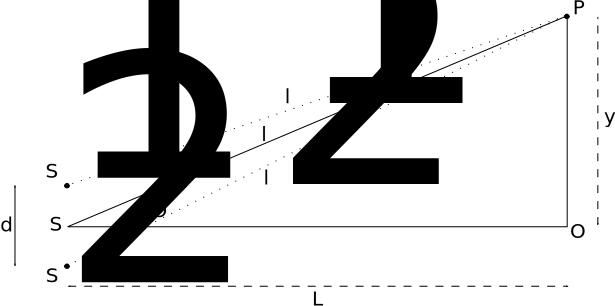
\includegraphics[width=2\textwidth/3]{figures/definitions}  
  \caption{The relationship between the two light sources, \Sone and
    \Stwo, and the screen $OP$, along with definitions of the various
    distances quoted in the text.}
  \label{fig:sources}
\end{figure}

Consider what happens if you have two coherent\footnote{Two sources
  are coherent if they emit the same frequency of light with a
  vanishing relative phase angle.} light sources, \Sone and \Stwo; see
Figure~\ref{fig:sources}.  Let's set them up so that the two sources
are a distance $d$ apart, and equidistant from a screen.  Assume the
distance from the screen to the sources, $L$, is much much larger than
their separation ($d\gg L$).  Wavefronts from the two waves will
completely constructively interfere at a point on the screen when the
light has to travel the same number of wavelengths from each source to
that point; there will be a bright spot on the screen at that point.
More generally, there will be a bright spots at every point on the
screen where the travel distances differ by an integer multiple of the
wavelength; similarly, complete destructive interference will occur if
the travel distances differ by an odd half-multiple of the wavelength
(0.5, 1.5, etc.).

Let's calculate where on the screen these bright spots will occur;
we'll use the notation in Figure~\ref{fig:sources}.  We can define the
location of the point $P$ by the $x$ and $y$ offsets ($L$ and $y$
respectively), as well as by the magnitude and angle ($\ell$ and
$\theta$).  Of course, they are related by $\tan\theta = y/L$.  Now,
we know that the points of constructive interference occur when
$\ell_2 - \ell_1 = n \lambda$, where $n$ is an integer and $\lambda$
is the wavelength of the sources.  We can calculate $\ell_1$ and
$\ell_2$ via the Pythagorean theorem
\begin{align*}
  \ell_1^2 &= \left(y - \frac{d}{2}\right)^2 + L^2 & 
  \ell_2^2 &= \left(y + \frac{d}{2}\right)^2 + L^2\ .
\end{align*}
Now, by assumption $d \ll L$, and we'll also assume $d \ll y$.  We can
use Taylor's theorem, and expand each of the parenthesized factors
\begin{gather*}
  \left(y - \frac{d}{2}\right)^2 =   y^2 \left(1 -
    \frac{d}{2y}\right)^2 \approx 
  y^2 - dy\ .
\end{gather*}
After expanding the similar terms in both of the $\ell_i$, you should
find
\begin{align*}
  \ell_1^2 & \ell^2 + L^2 - dy &
  \ell_2^2 & \ell^2 + L^2 + dy \ .
\end{align*}
Taking the difference of these terms gives
\begin{gather*}
  \ell_2^2 - \ell_1^2 = \left( ell_2 - \ell_1 \right) \left( ell_2 +
    \ell_1 \right) \approx \left( ell_2 - \ell_1 \right) 2 \ell = 2dy\ .
\end{gather*}
Divide both sides by $2\ell$, and substitute for the first term, and
you should find for the maxima
\begin{gather}
  n \lambda = \frac{dy}{\ell} = d \frac{y}{\sqrt{y^2 + L^2}} = d
  \sin\theta\ .
\label{eq:grating}
\end{gather}

With only two coherent sources, the pattern on the screen will vary
smoothly from one bright peak to the next dim valley to the next
bright peak; in other words, we won't just see very bright peaks with
no light in between them.  If, however, we were to add another pair of
sources, we would still get bright peaks according to
Equation~\eqref{eq:grating}, but the spaces in between would be darker
than in the two source case.  If we keep adding sources until we have
a very large number of them, we would \textit{still} find that we have
bright peaks according to Equation~\eqref{eq:grating}, but essentially
no light between those peaks; destructive interference between all
the additional sources would essentially cancel all the light.

So, how do we obtain a large number of coherent sources?  We don't.
Instead, we obtain a \textit{single} source, and we place an opaque
layer of material between it and the screen.  Then, we cut a series of
very fine, closely and regularly spaced, parallel lines through the
opaque material.  At each slit, the light will emerge \textit{as if}
is was emerging from an independent source.  The object we would have
constructed is called a \textit{diffraction grating}, and the spacing
between the \textit{line} of the grating is called the \textit{grating
  element}, or line spacing, $d$.

\section{Procedures}
\label{sec:procedures}

In the lab, there will be a number of gas discharge tubes, a
Helium-Neon laser, diffraction gratings, measuring equipment, and
various mounts and stands.  First, you'll use a Helium-Neon laser,
which operates at a well known wavelength, to determine the line
spacing for your grating.  Then, you'll use the grating to determine
the emission wavelengths for a number of elements in gas discharge
tubes. 

\subsection{Helium-Neon Laser}
\label{sec:laser}

\begin{figure}
  \centering
  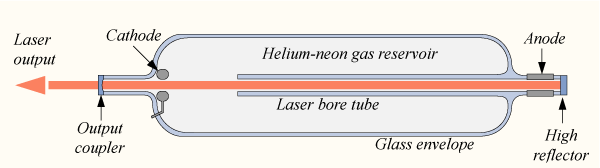
\includegraphics[width=2\textwidth/3]{figures/Hene-1}
%% From wikipedia: http://en.wikipedia.org/wiki/File:Hene-1.png
%% License: GFDL1.2 and CCASA3.0
  \caption{The construction of a Helium-Neon Laser consists of a gas
    discharge tube capped on each end with high-efficiency mirrors.}
  \label{fig:lasertube}
\end{figure}

\begin{figure}
  \centering
  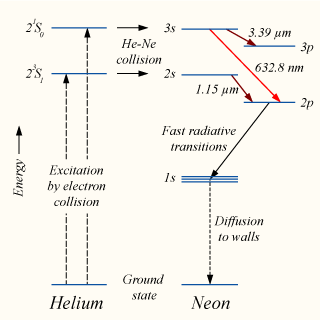
\includegraphics[width=2\textwidth/3]{figures/Hene-2}
%% From wikipedia: http://en.wikipedia.org/wiki/File:Hene-2.png
%% License: GFDL1.2 and CCASA3.0
  \caption{The level structure, and corresponding wavelengths, of the
    Helium-Neon laser system.}
  \label{fig:levels}
\end{figure}

The helium-neon, or HeNe, laser was among the first continuous lasing
systems ever developed.  It's cheap, efficient, and produces its
output in the optical part of the spectrum.  This lasing system is
essentially a gas discharge tube capped on each end with high
efficiently mirrors; see Figure~\ref{fig:lasertube}.  The discharge
excites Helium atoms to a set of long lived, metastable excited
states; collisional interactions transfer this energy to the Neon
atoms, exciting some of their electrons to the $^3s_2$ level.  These
transition to the $^2p_4$ state, emitting in the process a photon
whose wavelength in air at STP is \unit[632.816]{nm}.\footnote{The
  emitted wavelength is \unit[632.991]{nm} in vacuum.  Data gleaned
  from wikipedia.}  This is right in the middle of the red band of the
optical spectrum.

When we shine the laser through the grating, a single diffraction
pattern will form on the screen.  Since we can accurately measure the
angular divergence of the first order peaks, we can accurately
determine the grating element.  That's your goal in the first part of
the lab.

\begin{quote}
  \textbf{\textit{LASER SAFETY: Do not intentionally stare into the
      laser light! While a brief, inadvertent exposure to our HeNe
      lasers will not injure your eyes, intentionally staring into the
      beam for any length of time could give you anything from
      temporary vision impairment to permanent eye injuries, including
      blindness!}}
\end{quote}

You are going to shine the laser on the wall, through the grating, and
measure the positions of the zeroth and first order peaks.  This data
will give you the angle, and consequently, you can determine the
grating element.
\begin{enumerate}
\item Mount the laser so that it shines on the wall or chalkboard.
  The beam should meet the board at a right angle.
\item Mount the grating parallel to the wall, so that the laser shines
  through it.  Locate the first order peaks; the lights in the room
  will probably need to be off for this.
\item Carefully measure the distance from the grating to the wall
  ($L$), and the distance from the zeroth order peak to both first
  order peaks ($y_1$ and $y_{-1}$).  The latter two should be the
  same; if they are not, either your beam is not normal to the wall,
  or your grating is not parallel to the wall.  
\item Record these numbers carefully, and determine the grating
  element. 
\end{enumerate}

Now that you have the grating element, you can use your grating to
determine the wavelengths of any number of light sources.

\subsection{Laser Pointers}
\label{sec:pointers}

The red laser pointer uses a solid state laser diode to produce a beam
in the optical spectrum.  The exact wavelength is highly variable, and
depends on the exact composition of the semiconductor diode, the
coatings on the lenses in the optical system, and the temperature of
the electronics.  Still, they are \textit{red}, and they are
\textit{lasers}, so the range of wavelengths output by a given pointer
are very narrow.  Determine the wavelength of your pointer.

\begin{enumerate}
\item Repeat the measurement of the previous section, but using a
  laser pointer instead of the HeNe laser unit.  
\item Record $L$, $y_1$, and $y_{-1}$, and determine the wavelength
  the laser pointer.
\end{enumerate}

\subsection{Gas Discharge Tubes}
\label{sec:tubes}

In a gas discharge tube, a low pressure gas is ionized by a high
voltage current flowing between two electrodes.  The recombination of
electrons onto the atoms results in the emission of specific
wavelengths of electromagnetic radiation.  Fluorescent lights are the
most commonly encountered form of gas discharge tubes.  They use
mercury vapor, which emits a number of lines in the ultraviolet region
of the spectrum to excite fluors coated on the inside surface of the
glass, which then fluoresce across the optical band.

In contrast, we will study pure gasses in this lab, which will show us
the behavior of specific atomic species.  Some of these emission lines
are in the optical region of the spectrum.  Since these emission lines
contain a vary narrow range of wavelengths, we can use a diffraction
grating to determine the wavelengths of these lines.  Different color
light (different wavelengths) will be diffracted through different
angles, much like in a prism.  How does the ordering of colors compare
with those in a prism?

\begin{quote}
  \textbf{\textit{DISCHARGE TUBE SAFETY: These operate with a very
      high voltage between their terminals.  Do NOT stick your
      fingers, pens, etc. into the terminals.  Do NOT touch the ends
      of the tube when they are on.  Do NOT remove the tubes when they
      are energized. Do NOT leave them on for more than a minute at a
      time.  Also, the tubes get HOT when run for more than a few
      seconds; don't touch then until they have cooled down.}}
\end{quote}

Unlike the laser measurements made in the first two parts of the lab,
the light from the discharge tubes is neither coherent, nor focused,
and hence can't form an image on a screen or wall.  Instead, you will
be using your personal optical measurement system (ie, your retina) as
the screen.  This type of image is called a \textit{virtual} image.
\begin{enumerate}
\item Fix a meter stick in the horizontal, and set a discharge tube
  vertically at the midpoint of the stick, and as close to the stick
  as possible.  Mount the grating at a suitable distance (something
  like \unit[50]{cm} should work) from the meter stick, with the
  grating lines parallel to the length of the discharge tube.  Make
  sure grating is parallel to both the meter stick and the tube.
\item Look through the grating towards the discharge tube; keep your
  eye as close to the grating as possible to eliminate parallax
  shifts.  Find the spectral lines, which will appear on both sides of
  the central maximum.  If you did the previous step correctly, they
  should be symmetric about the central maximum.  Adjust the distance
  so that the furthest first order line is as far out on the meter
  stick as possible.  
\item Record the type of gas in the tube.  Measure and record the
  distance from the discharge tube to the grating.  Measure and record
  the colors and positions on the meter stick of all the first order
  lines on both sides of the central maximum.
\item Repeat with another gas.
\end{enumerate}

\newpage
 
\section*{Pre-Lab Exercises}

Answer these questions as instructed on Blackboard; make sure to
submit them before your lab session!

\begin{enumerate}
\item Why is the zeroth order maximum the same color as the source?
  For lines of a given order, are the red or violet lines on the
  screen closer to the zeroth order maximum?
\item What wavelength of light would produce a first order peak at
  10\textdegree with a grating of $10^4$ lines per centimeter?
% 174nm
\item A $\unit[340]{n m}$ wave with a grating of 5,000 lines per
  centimeter produces its first order peak at what angle?
% 9.8\textdegree
\item Determine the grating element for a wavelength of
  $\unit[500]{n m}$ to produce a second order peak at 15\textdegree.
% 2590/cm, 3.8e-6m
\end{enumerate}

\newpage

\section*{Post-Lab Exercises}

\begin{enumerate}
\item From your HeNe data in Section~\ref{sec:laser}, determine the
  grating element for your grating.  Since both of your first order
  measurements should give the same result, combining them should give
  you a more accurate measurement.  Estimate the uncertainty of your
  measurement.
\item From your data in Section~\ref{sec:pointers}, determine the
  wavelength of you laser pointer.  Estimate the uncertainty of your
  measurement.  Remember that the HeNe laser is also \textit{red}, so
  the wavelengths won't be too far off.  Don't forget to combine the
  data from both first order measurements.
\item For each of the gasses you measured in Section~\ref{sec:tubes},
  determine all the first order line wavelengths.  Estimate the
  uncertainties.  Don't forget to combine the data from both first
  order measurements.  These wavelengths are all well measured; look
  them up.  How well do your measured values match the tabulated
  results? 
\item Discuss briefly whether you have met the objectives of the lab
  exercises.
\end{enumerate}

\end{document}


From \url{http://hyperphysics.phy-astr.gsu.edu/hbase/hyde.html} The
measured lines of the Balmer series of hydrogen in the nominal visible
region are:

\begin{tabular}{|cccl|}\hline
  Wavelength [\unit{nm}] & Relative Intensity & Transition &
  Color\\\hline 
  383.5384 	& 5 &	$9 \to 2$ & Violet\\
  388.9049 	& 6 &	$8 \to 2$ & Violet\\
  397.0072 	& 8 &	$ 7 \to 2$ & Violet\\
  410.174 	& 15 &	$6 \to 2$ & Violet\\
  434.047 	& 30 &	$5 \to 2$ & Violet\\
  486.133 	& 80 &	$4 \to 2$ & Blue-green (cyan)\\
  656.272 	& 120 &	$3 \to 2$ & Red\\
  656.2852 	& 180 &	$3 \to 2$ & Red\\\hline
\end{tabular}

The red line of deuterium is measurably different at 656.1065 (
\unit[.1787]{nm} difference).





Helium data from
\url{http://hyperphysics.phy-astr.gsu.edu/hbase/quantum/atspect.html}
which references ``Jenkins and White, Ch. 21''.

\begin{tabular}{|cl|}\hline
  Wavelength [\unit{nm}] & Relative Intensity\\\hline
  438.793 & weak\\
  443.755 & weak\\
  447.148 & strong\\
  471.314 & medium\\
  492.193 & medium\\
  501.567 & strong\\
  504.774 & weak\\
  587.562 & strong\\
  667.815 & medium\\\hline
\end{tabular}



Mercury, from
\url{http://webphysics.davidson.edu/course_material/py230l/spectra/spectra.htm}
and
\url{http://hyperphysics.phy-astr.gsu.edu/hbase/quantum/atspect2.html#c1}.
there are other weak lines not tabulated here.

\begin{tabular}{|cl|}\hline
  Wavelength [\unit{nm}] & Color\\\hline
  404.656 & Violet\\
  435.835 & Blue\\
  546.074 & Green\\
  576.959 & Yellow\\
  579.065 & Yellow\\\hline
\end{tabular}




Sodium, from
\url{http://hyperphysics.phy-astr.gsu.edu/hbase/quantum/sodium.html}

\begin{tabular}{|cccl|}\hline
  Wavelength [\unit{nm}] & Relative Intensity & Transition &
  Color\\\hline 
  588.9950 & 2 & $3p_{3/2} \to 3s_{1/2}$ & Yellow\\
  589.5924 & 1 & $3p_{1/2} \to 3s_{1/2}$  & Yellow\\\hline
\end{tabular}


%%% Local Variables: 
%%% mode: latex
%%% TeX-master: t
%%% End: 
